\section{Tell Me Something New}\label{sec:tmsn}
We start with a general description of \tmsn\ which will be followed
by a description of \tmsn\ for boosting. To streamline our presentation
we consider binary classification, but other supervised or
unsupervised learning problem can be accommodated with little change.

We are given
\newcommand{\cD}{{\cal D}}
\begin{itemize}
\item A set of classifiers $\strongRules$, each classifier $H \in
  \strongRules$ is a mapping from an input space $X$ to a binary label $\{-1,+1\}$.
\item A stream of labeled examples $(x_1,y_1),(x_2,y_2),\ldots$, $x_i
  \in X$, $y_i \in \{-1,+1\}$, generated IID according to a fixed but
  unknown distribution $\cD$.
\end{itemize}

The goal of the algorithm is to find a classifier $H \in
\strongRules$ that minimized the error probability $\err(H)\doteq
P_{(x,y) \sim \cD}[H(x) \neq y]$

All workers start from the same initial classifier $H_0$ which is
improved iteratively. Some iterations end with the worker finding a
better classifier by itself, others end with the worker receiving a
better classifier from another worker. The sequences of classifiers
corresponding to different workers can be different, but with high
probability they all converge to the same classifier.

Denote each worker by an index $i=1,\ldots,n$. On iteration $t$
each worker has its {\em current} classifier  $H_i(t)$ and a set of $m$
{\em candidate} classifiers $G_i^j(t)$. An error upper bound
$\errub(H_i(t))$ is associated with $H_i(t)$ so that with high
probability $\errub(H_i(t)) \geq \err(H_i(t))$.

\begin{figure}[t]
%\begin{minipage}{.31\textwidth}
\begin{center}
  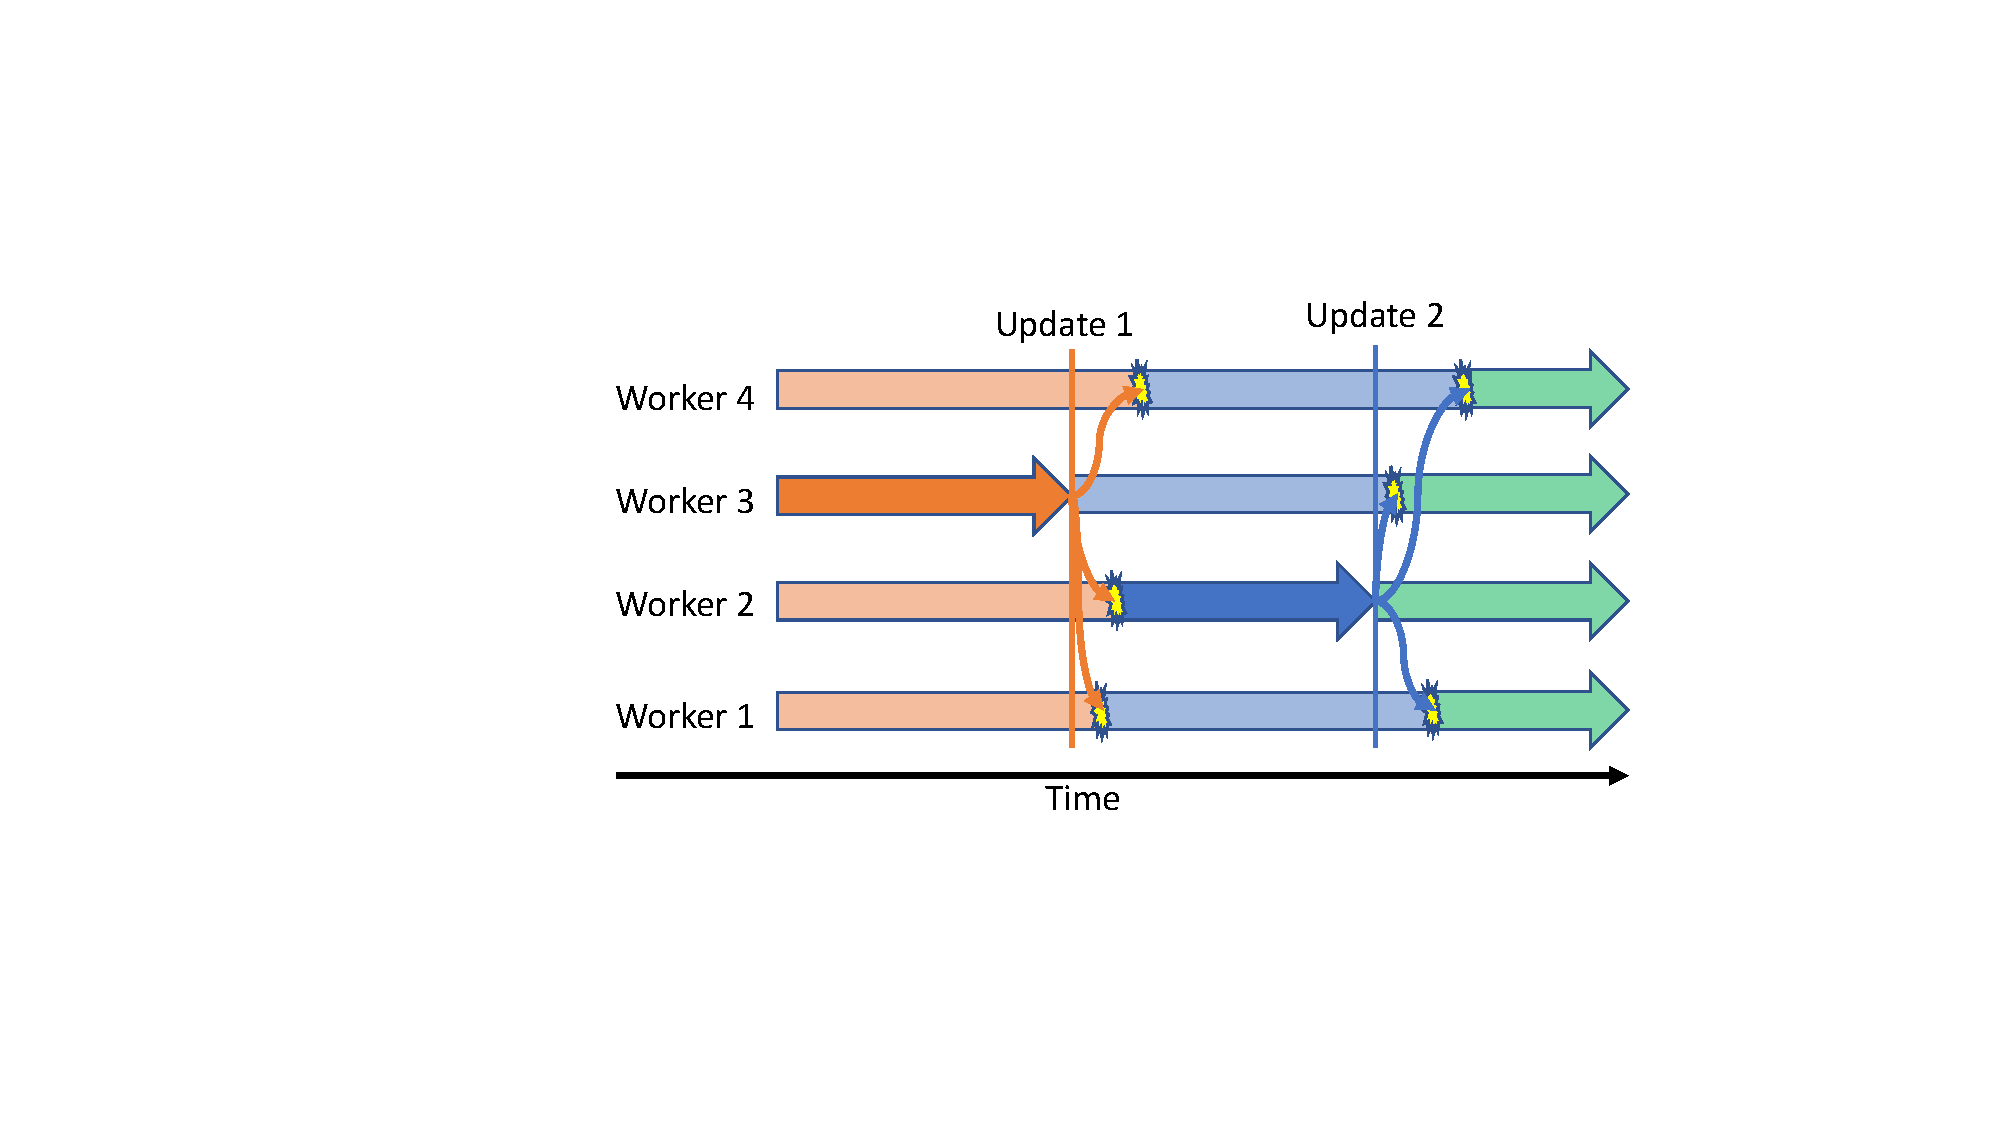
\includegraphics[width=0.7\textwidth]{AsyncUpdates.pdf}
\end{center}
  \caption{{\bf Execution timeline of a \tmsn\ system}
      System consists of four workers. The first update occurs when
      worker 3 identifies a better classifier $H_1$. It then replaces
      $H_0$ with $H_1$ and broadcasts $(H_1,z_1)$ to the
    other workers. The other workers receive the message the at different
    times, depending on network congestion. At that time they  interrupt the
    scanner (yellow explosions) and start using $H_1$. Next, worker 2
    identifies an improved rule $H_2$ and the same process ensues.
    \label{fig:async}}
   	\vspace{0pt}
%\end{minipage}
\end{figure}

The worker reads examples from the stream and uses them to estimate
the errors of the candidates. It stops when it finds a candidate that,
with high probability, has an error smaller than
$\errub(H_i(t))-\epsilon$ for some constant ``gap'' parameter
$\epsilon>0$.

More precisely, the worker uses a {\em stopping rule} that chooses a
stopping time and a candidate rule and has the property that, with
high probability, the chosen candidate rule has an error smaller than
$\errub(H_i(t))-\epsilon$. This candidate then replaces the current
classifier, the new upper bound is set to be $\errub(H_i(t+1)) =
\errub(H_i(t))-\epsilon$, a new set of candidates is chosen and the
worker proceeds to the next iteration. At the same time the worker
{\em broadcasts} the pair $(H_i(t+1), \errub(H_i(t+1))$.

A separate process in each worker listens to broadcasts of this
type. When worker $i$ receives a pair $(H,\errub(H))$ it compares the
upper bound $\errub(H)$ with the upper bound associated with it's
current classifier $\errub(h_i(t))$. If $\errub(H) < \errub(h_i(t))-\epsilon$,
it interrupts the current search and sets $H_i(t+1)=H$. If not the
received pair is discarded.

Note that the only assumption that the workers make regarding the
incoming messages is that the upper bound $\errub(H)$ is sound. In
other words that, with hight probability, it is an upper bound on the
true error $\err(H)$. There is no synchronization and if a worker is
slow or fails, the effect on the other workers is minimal.

Different implementations of \tmsn\ differ in the way that they
generate candidate classifiers and in the stopping rules that they
use. For \tmsn\ to be effective, the stopping rule should be both
sound and tight. If it is not sound, then the scheme falls apart, and
if it is not tight, then the stopping rules stop later than needed,
slowing down convergence.

Next, we describe how \tmsn\ is applied to boosting.
